\documentclass[authoryear, review, 11pt]{elsarticle}

\setlength{\textwidth}{6.5in}
%\setlength{\textheight}{9in}
\setlength{\topmargin}{0in}
\setlength{\oddsidemargin}{0in}
\setlength{\evensidemargin}{0in}

\usepackage{amsmath}
\usepackage{amsthm}
\usepackage{amssymb}
\usepackage{mathabx}
\usepackage{bm}
\usepackage{multirow}

%\geometry{landscape}                % Activate for for rotated page geometry
\usepackage[parfill]{parskip}    % Activate to begin paragraphs with an empty line rather than an indent
\usepackage{graphicx}
\usepackage{epstopdf}
\usepackage{natbib}
\usepackage{verbatim}

\usepackage{endfloat}

\usepackage{relsize}
\usepackage{caption}
\usepackage{subcaption}
%\usepackage{fullpage}
\usepackage{booktabs}

\DeclareGraphicsRule{.tif}{png}{.png}{`convert #1 `dirname #1`/`basename #1 .tif`.png}
\DeclareMathOperator*{\argmin}{\arg\!\min}
\DeclareMathOperator*{\argmax}{\arg\!\max}
\DeclareMathOperator*{\bw}{\mbox{bw}}
\DeclareMathOperator*{\df}{\mbox{df}}
\newcommand{\vect}[1]{\bm{#1}}
\newcommand{\E}{\mathop{\mathbb E}}


\title{Modeling PalEON biomass}
\author{Wesley Brooks}
\date{}                                           % Activate to display a given date or no date

\begin{document}
\maketitle
%\section{}
%\subsection{}


\section{Introduction}
Our objective is a  model of the biomass of each species in each grid cell, where the only parameters used to calibrate the models are location and species composition. It is important to come up with an estimated probability that a given cell will have no biomass of a given species, and also to model the variance of the biomass estimate.


\section{Philosophy}
Jun and I discussed the interpretation of a model for biomass. At the time I saw the effort being directed toward getting a model that tells us, based on our survey of the forests at time of settlement, how much biomass there was on the landscape at time of settlement. On the other hand, Jun says that the goal is to model the process that gives rise to biomass on the landscape, observed through the survey at time of settlement.

As a practical matter, one implication is that grid cells where there were small but nonzero biomass observations are treated differently. In my view, the fact that, say, a spruce tree was seen in grid cell 517 is enough to say that there is zero probability of there being no spruce biomass in cell 517. In Jun's view, we could easily imagine the same process populating the landscape in such a way that, randomly, cell 517 has no spruce trees. So there's a positive probability of zero spruce in cell 517.


\section{Models}
There are two possible directions here: a two-stage hierarchical model, where in stage one we randomly decide whether a given cell has nonzero biomass, and then if so stage two randomly sets the biomass; alternatively, a single-stage model with zero-inflation, maybe one that could be tuned like a \verb!glm! (e.g. a Tweedie model).


\section{Figures}
\begin{figure}
	\begin{center}
	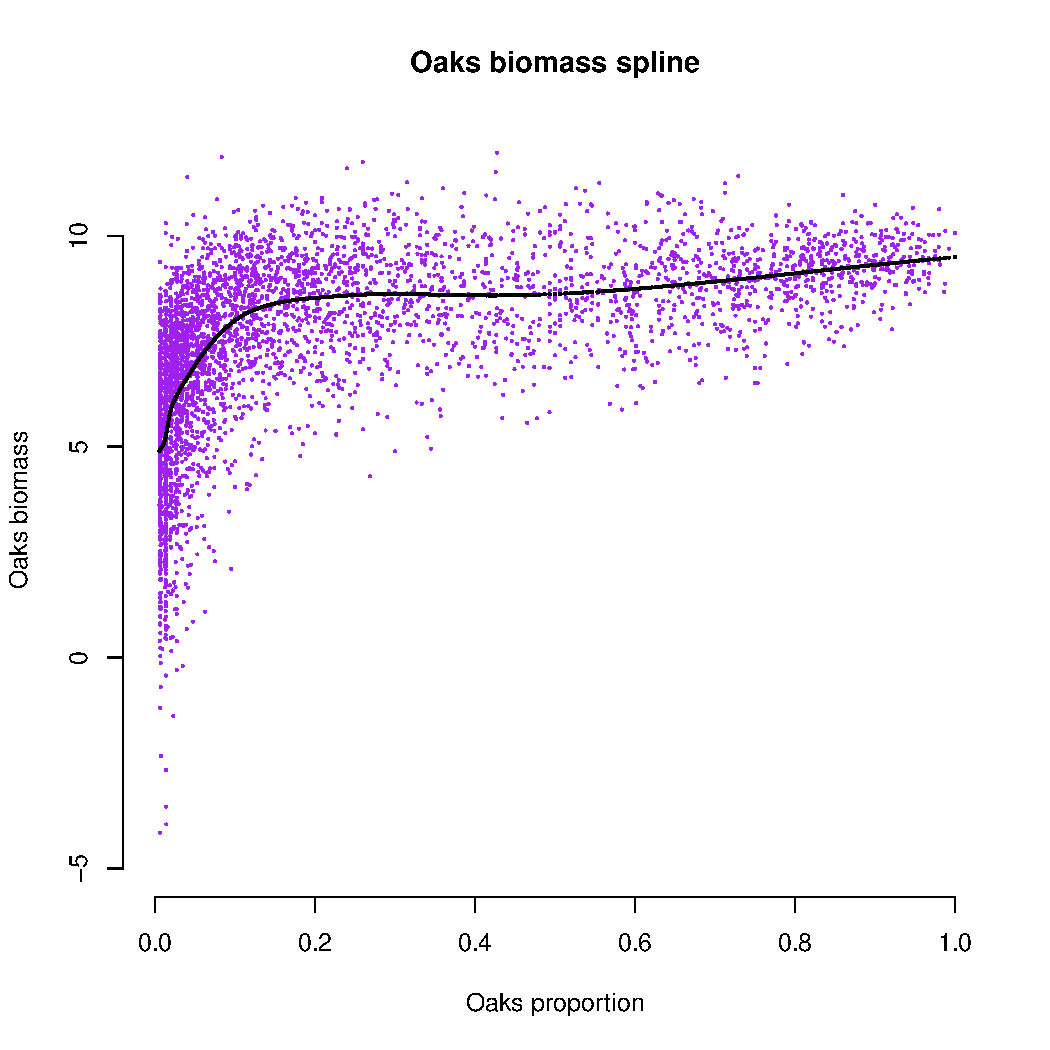
\includegraphics[width=5in]{../../figures/Oaks-biomass-spline.pdf}
	\end{center}
\end{figure}

\begin{figure}
	\begin{center}
	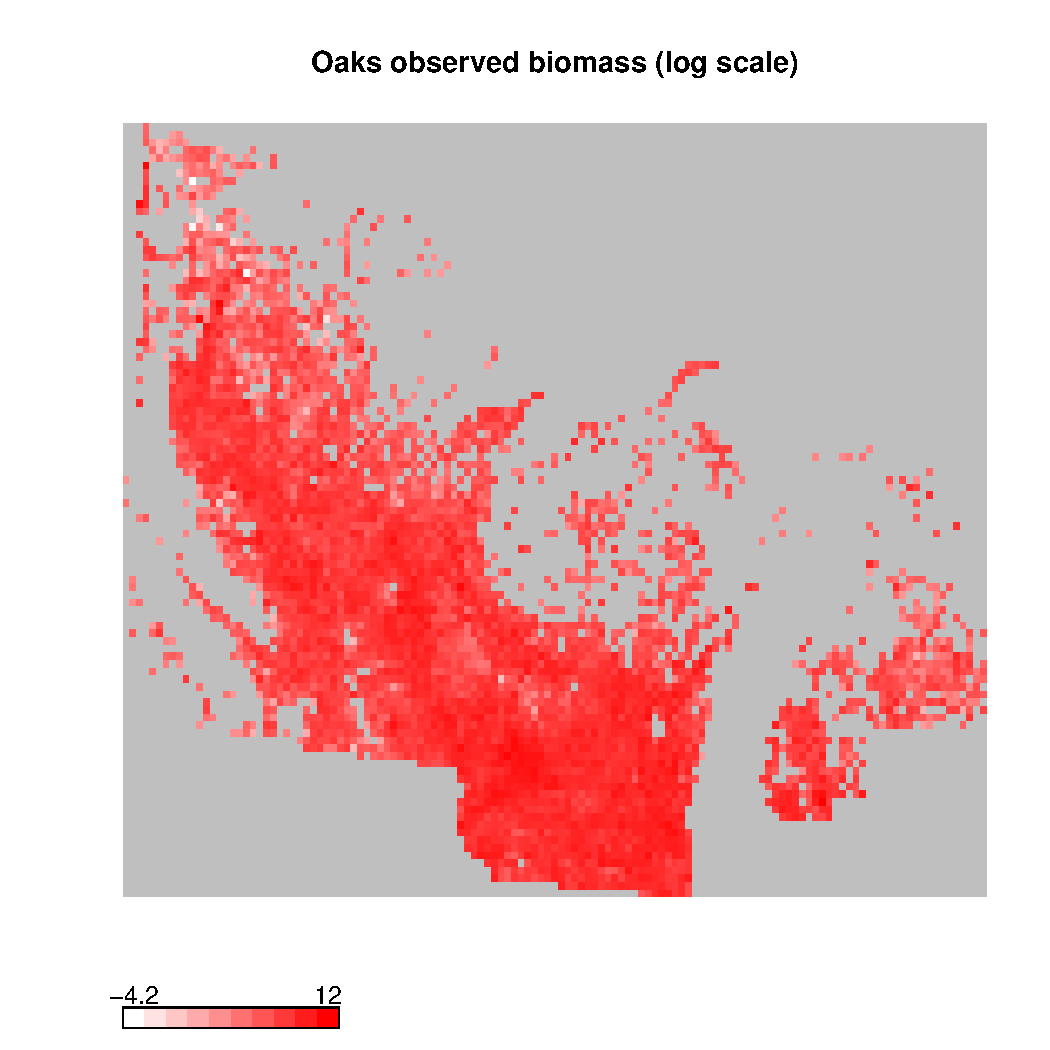
\includegraphics[width=5in]{../../figures/Oaks-biomass-observed.pdf}
	\end{center}
\end{figure}

\begin{figure}
	\begin{center}
	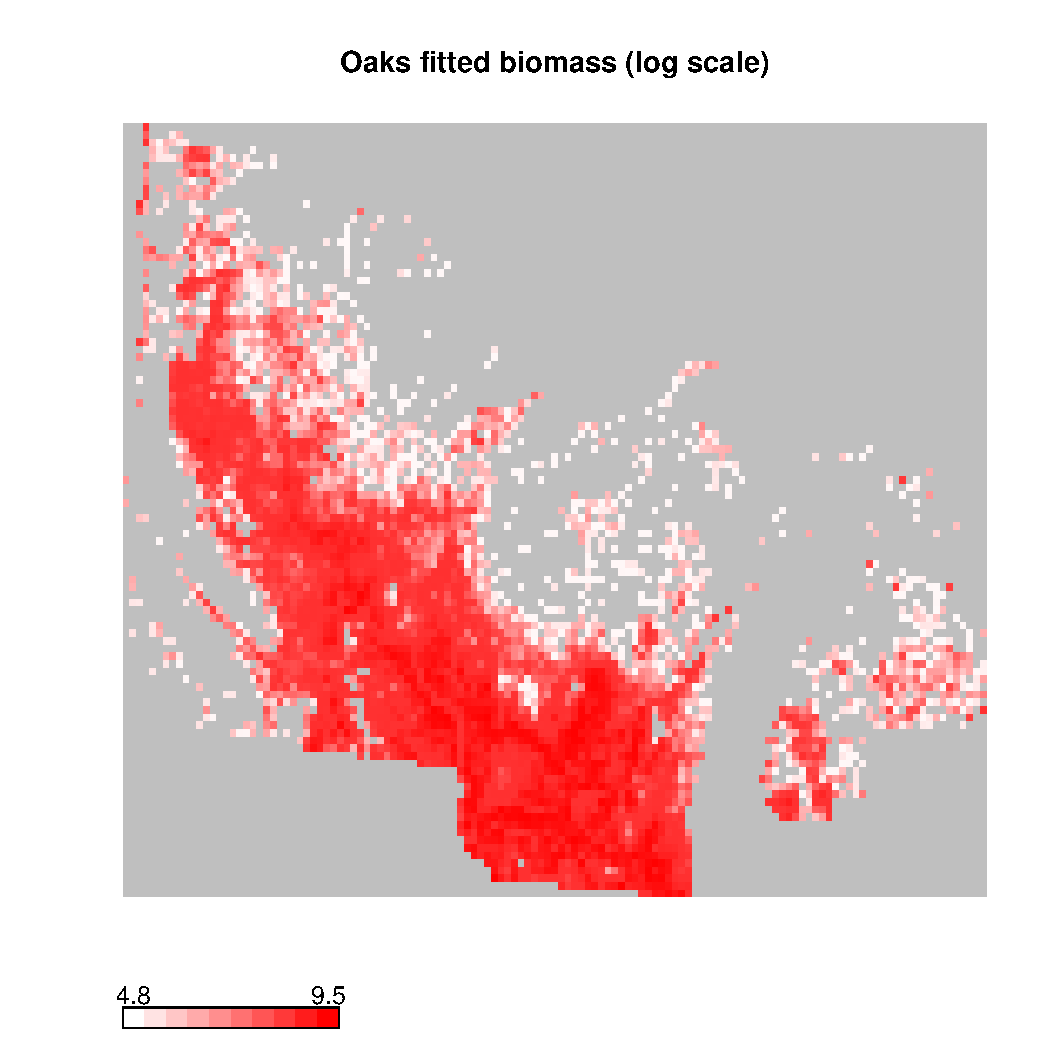
\includegraphics[width=5in]{../../figures/Oaks-biomass-fitted.pdf}
	\end{center}
\end{figure}

\begin{figure}
	\begin{center}
	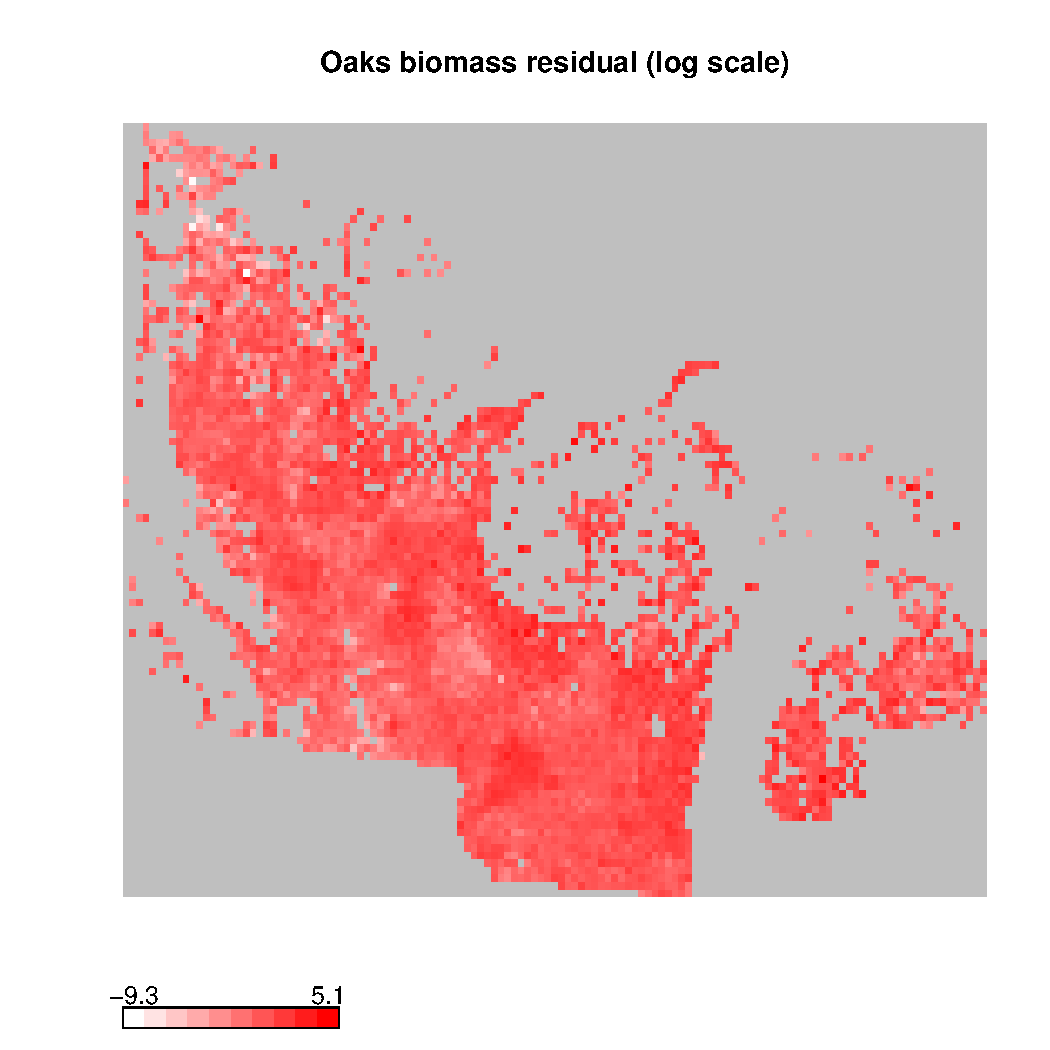
\includegraphics[width=5in]{../../figures/Oaks-biomass-residual.pdf}
	\end{center}
\end{figure}

\section{References}
%\bibliographystyle{chicago}
%\bibliography{../../references/biomass}

\end{document}  